\section{Verwendete Methoden Maschinellen Lernens}
\label{sec:lerner}
Zum Verständnis der Ergebnisse müssen zunächst die verwendeten 
Lerner und Methoden erläutert werden, die zur Klassifikation 
und Bewertung der Ergebnisse verwendet werden.

\subsection{Nächste-Nachbarn-Klassifikation}

Der k-Nächste-Nachbarn Klassifikator ist einer der einfachsten Lerner zur 
Klassifikation. Die Klassen werden zugeordnet, in dem die $k$ nächsten Nachbarn 
betrachtet werden. Dabei werden Abstandsmaße verwendet, wie beispielsweise 
euklidische Abstände. Die Wahl des Parameters $k$ hat dabei einen hohen Einfluss 
auf das Ergebniss, da ein zu geringer Wert hohe Sensitivität gegenüber Ausreißern 
hat und ein zu hoher Wert, viele Einträge aus anderen Klassen beinhalten kann. 
In Abbildung \ref{fig:knn} wird die Beeinflussung der Wahl der Anzahl der Nachbarn 
verdeutlicht.

\begin{figure}
  \centering
  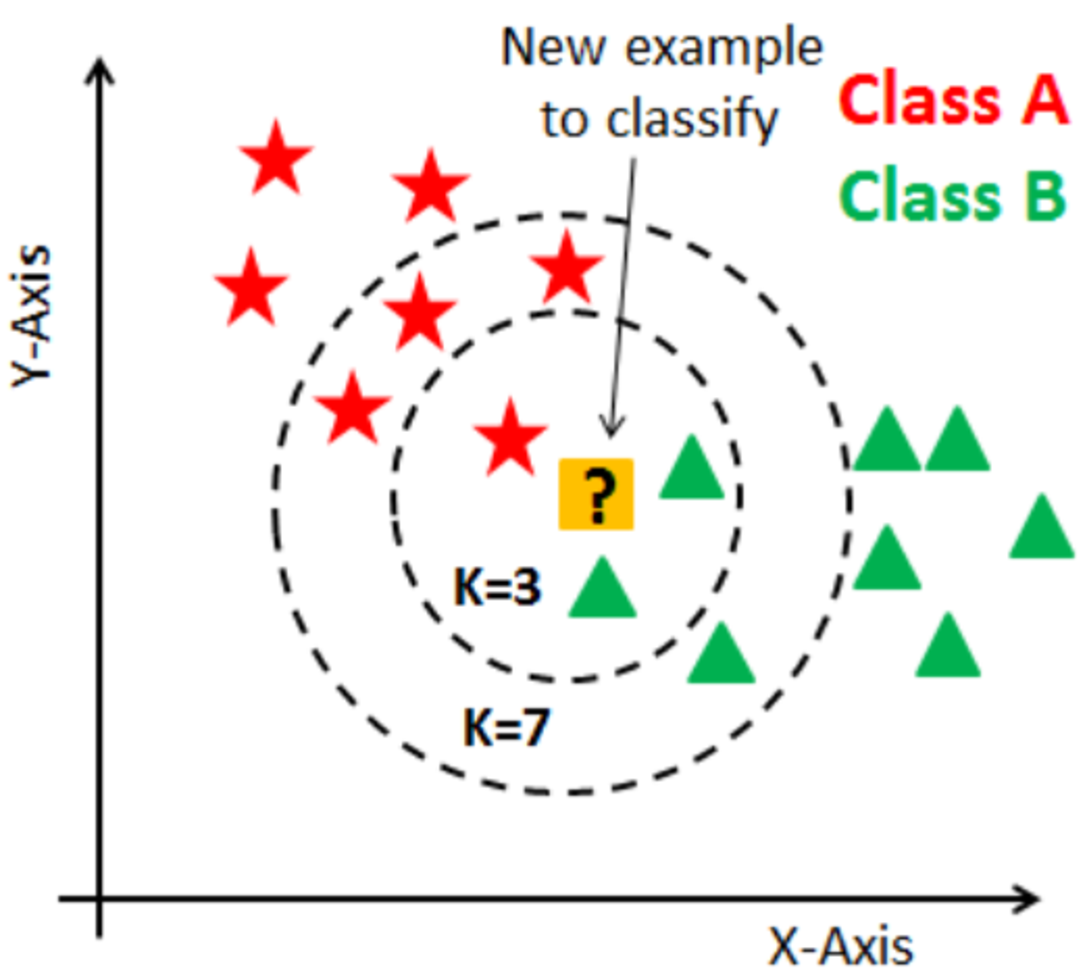
\includegraphics[width=0.5\textwidth]{plots/knn.pdf}
  \caption{Darstellung, wie die Wahl der Anzahl der Nachbarn die Klassifikation des Punktes 
  beeinflussen kann. Bei $k = 3$ wird der Punkt Klasse B zugeordnet. Bei 
  $k = 7$ wird der Punkt Klasse A zugeordnet \cite{kNN}.}
  \label{fig:knn}
\end{figure}

Ein
wichtiger Punkt des kNN-Lerners ist, dass er ein sogenannter \textit{lazy learner} 
ist. Das bedeutet, beim Trainieren werden die Daten lediglich abgespeichert und 
die Klassifikation findet nicht zeitgleich oder im Anschluss an das Training 
statt, sondern erst, wenn die Klassifikation angefordert wird. 


\subsection{Random Forest Klassifikationsverfahren}
Der \texttt{RandomForestClassifier} basiert auf binären Entscheidungsbäumen.
Bei einem Entscheidungsbaum wird an jedem Knoten ein Schnitt in einer Variable durchgeführt und die daraus entstandenen Teilmengen 
werden in den beiden Ästen des Knotens wiederum durch Schnitte unterteilt, bis entweder eine bestimmte Tiefe
des Baumes erreicht ist oder die Blätter nur Ereignisse einer Klasse enthalten. Um die Effekte des Übertrainierens zu minimieren, wird über ein Ensemble unterschiedlicher
Entscheidungsbäume gemittelt.
Die Bäume werden dabei jeweils auf unterschiedlichen Teilmengen des Trainingsdatensatzes trainiert.
Die Attribute des Baumes an denen der beste Schnitt gesucht wird, werden zufällig ausgesucht.

\subsection{Naive-Bayes-Klassifikator}
Der Naive-Bayes Klassifikator beruht auf dem Satz von Bayes, der lautet:

\begin{equation*}
    p\left(A|B \right) = \frac{p\left(B|A \right) p\left(A \right)}{p\left(B \right)} \, .
\end{equation*}

Dabei kann $A$ der Klassenzugehörigkeit entsprechen, wobei gilt, dass 
$A$ das Signal representiert und $\bar{A}$ den Untergrund. $B$ ist dann ein 
Attribut. Der Klassifikator beruht auf der Annahme, dass die Attribute bedingt 
unabhängig sind. Der Naive Bayes Lerner bestimmt die Wahrscheinlichkeit einer 
Klasse durch Beobachtungen. Für das Beispiel der Attributswahl für 
mehrere Attribute bei Signal und 
Untergrund gilt, dass

\begin{equation*}
    Q = \prod\limits_{i = 1}^{n} \frac{p\left(B_i|A \right)}{p\left(B_i|\bar{A} \right)}
\end{equation*}
größer als Eins ist, wenn das Ereignis eher Signal als Untergrund entspricht. 
Für $Q \textless 1$ gilt, dass das Ereignis wahrscheinlicher dem Untergrund 
zugeordnet werden kann.

\subsection{Qualitätsparameter}
In der Analyse werden verschiedene Parameter verwendet um die Qualität der Klassifizierung 
und die Stabilität der Attributsauswahl zu bewerten. Die dabei wichtigen Parameter 
sind die Reinheit, die Effizienz und der Jaccard-Index. \par 
Für die Berechnung der Reinheit und der Effizienz werden Werte benötigt, die 
eine richtige oder falsche Einordnung identifizieren. Wird ein Ereignis dem 
Parameter \textit{true positive $tp$} zugeordnet, bedeutet das beispielsweise,
dass die Zahl korrekt als Signal eingeordnet wurde. \textit{False positive $fp$} 
bedeutet, die Zahl wurde als Signal eingeordnet, ist aber eigentlich ein
Untergrund. Als \textit{true negative $tn$} gilt eine Zahl, die richtig dem Untergrund 
zugeordnet wurde und \textit{false negative $fn$} beschreibt ein Signal, welches 
fälschlicherweise dem Untergrund zugeordnet wurde. Die Reinheit und die Effizienz 
berechnen sich dann nach:

\begin{align*}
    \text{Reinheit}\, \, p &= \frac{tp}{tp + fp} \\ 
    \text{Effizienz}\, \, r &= \frac{tp}{tp + fn} \, .\\ 
\end{align*}

Der Jaccard-Index beschreibt die Stabilität der Attributsauswahl gegen statistische 
Schwankungen im Lerner. Er wird berechnet über 

\begin{equation*}
    J \left(F_a, F_b \right) = \frac{|F_a \cup F_b|}{|F_a \cap F_b|}
\end{equation*}
und beschreibt die Ähnlichkeit der beiden Mengen $F_a$ und $F_b$. Zur Bewertung 
gilt dann: 

\begin{equation*}
    \hat{J} = \frac{2}{l \left(l - 1 \right)} \sum\limits_{i = 1}^{l}\sum\limits_{j = i+1}^{l} J\left(F_i, F_j \right) \, .
\end{equation*}
Qualitativ bedeutet das, dass die Attributsauswahl $l$-mal auf $l$ Teilmengen des Datensatzes durchgeführt wird. Der Index 
selber 

\subsection{Kreuzvalidierung}

Kreuzvalidierung wird benötigt, um einen Fehler auf die Qualitätsparameter angeben zu 
können.

\subsection{ROC-Kurven}